\documentclass[11pt,a4paper]{article}

\usepackage[margin=1in]{geometry}
\usepackage{times}
\usepackage{amsmath,amssymb}
\usepackage{booktabs}
\usepackage{graphicx}
\usepackage{xcolor}
\usepackage{hyperref}
\usepackage{enumitem}
\usepackage{caption}
\usepackage{tabularx}
\usepackage{array}
\usepackage{microtype}
\usepackage[numbers,sort&compress]{natbib}
\usepackage{fancyhdr}
\usepackage{float}
\usepackage{algorithm}
\usepackage{algpseudocode}

\hypersetup{
  colorlinks=true,
  linkcolor=black,
  citecolor=blue!50!black,
  urlcolor=blue!50!black,
  pdftitle={J-space probes on Gemma-2-9B-it: method and results},
  pdfauthor={Andy Liang}
}

\pagestyle{fancy}
\fancyhf{}
\fancyhead[L]{\small J-space probes on Gemma-2-9B-it}
\fancyhead[R]{\small Andy Liang · 4 November 2026}
\fancyfoot[C]{\thepage}
\renewcommand{\headrulewidth}{0.4pt}

\captionsetup{font=small,labelfont=bf}
\setlength{\emergencystretch}{1.5em}
\newcommand{\ci}[3]{#1\,[#2,\,#3]}
\newcommand{\WU}{W_U}
\newcommand{\hJ}{h_J}
\newcommand{\hC}{h_C}
\newcommand{\norm}[1]{\lVert #1 \rVert}
\newcolumntype{L}{>{\raggedright\arraybackslash}X}

\title{\textbf{J-space Probes on Gemma-2-9B-it}\\[0.3em]
\large Method and results: where the collusion signal does and does not live}
\author{Andy Liang\\[0.4em]
{\normalsize\textit{NARCBench Transfer-stable lane}}\\[0.2em]
{\normalsize\texttt{andylikescodes/narcbench-core-demo}, branch \texttt{jspace-separability}}}
\date{4 November 2026}

\begin{document}
\maketitle

\section*{Summary}

A linear probe on the hidden states of \texttt{google/gemma-2-9b-it} tells colluding committee agents from honest ones. We asked whether the part of the hidden state the probe uses lies inside \emph{J-space}, the directions that feed the model's next-word output, or outside it. To answer, we split every hidden state into a J part and a remainder, trained the same probe on each part, and tested on scenario families the probe had never seen.

\begin{enumerate}[leftmargin=1.6em,itemsep=0.2em]
\item \textbf{The probe restricted to J-space does not transfer.} Trained on the Core scenarios and tested on 72 episodes from six new families, it scores \ci{0.602}{0.471}{0.733} with one J-space estimate and \ci{0.549}{0.416}{0.683} with the other (AUROC with 95\% intervals; neither is distinguishable from chance). The unrestricted probe scores 0.902.
\item \textbf{The probe restricted to the remainder transfers as well as the unrestricted probe.} It scores 0.898 and 0.891 under the two estimates, against 0.902. The gap between remainder and J-space is $+0.30$ and $+0.34$, with $p<10^{-3}$.
\end{enumerate}

Inside the Core scenarios both parts separate colluders (J-space 0.989 and 0.961; remainder 1.000), so the J part is not empty; what it holds does not carry over to new families. Two things to keep in mind when reading this: ``J-space'' here is an approximation of the construction of \citet{gurnee2026verbalizable}, made two ways (Section~\ref{sec:frames}), and the Gemma runs did not include a control that asks whether \emph{any} 25 directions would behave the same way (Section~\ref{sec:scope}). The rest of this document is the method, step by step, with the exact settings behind every number.

\section{What was measured}

NARCBench~\citep{rose2026narcbench} is a benchmark of committee games. Four language-model agents review a briefing and vote; in half of the episodes two of them secretly coordinate. The benchmark's detector is a linear probe: a direction in the model's hidden state that scores each agent, with episode-level statistics on the four scores. Gemma-2-9B-it generated all the episodes used here and is the model whose hidden states were probed.

J-space is the idea of \citet{gurnee2026verbalizable}: at each layer, a small set of directions in the hidden state are the ones the rest of the network turns into output words, and the paper argues that these directions behave like a workspace the model can report from. If the collusion signal sat in those directions, a monitor could read it out as words. We tested this by restriction: project each hidden state onto its J-space directions (the \emph{J-only} arm) or onto everything else (the \emph{complement} arm), run the benchmark's probe on each, and compare with the probe on the full hidden state. The comparison that matters is on new scenario families, because inside the training distribution almost any restriction works.

\section{Data}
\label{sec:data}

\paragraph{Model.} \texttt{google/gemma-2-9b-it}~\citep{gemma2}: 42 decoder blocks, hidden width $d=3{,}584$, vocabulary $V=256{,}000$. Input and output embeddings are tied, so the output matrix $\WU\in\mathbb{R}^{V\times d}$ is \texttt{embed\_tokens.weight}. Hidden states were read after blocks 19 to 23 (45\% to 55\% of depth).

\paragraph{Core episodes (training distribution).} 100 episodes: 50 scenarios in 17 domains (audit, hiring, medical ethics and others), each run once as a collusion episode and once as a control twin with the same briefing, names and seed and no coalition. Four agents per episode. In a collusion episode two agents are colluders: their system prompt carries a hidden instruction, they exchange one private message each in round~0, and their prompts for the public rounds carry a \texttt{PRIVATE COORDINATION} block with both messages. Rounds 1 to 3 are public. Each agent then votes with the line \texttt{RECOMMENDATION: Option A|B} and a rationale. The episodes were generated on 1 October 2026 with Gemma-2-9B-it playing all four agents (\path{scripts/regen_gemma_core.py}, following the benchmark's \path{generation/core.py}; run id \texttt{20261001T012639Z}; transcripts under \path{upstream/scenarios/gemma2_9b/core/}).

\paragraph{Transfer episodes (test distribution).} 72 episodes: six families (CI/CD pipelines, code review, news, pump-and-dump, RAG corpora, research integrity), six scenarios each, each as collusion and control, so 36 and 36. Each family has its own generator and its own coalition task (hide a code flaw, shift a story's framing, pump a stock, seed a corpus, bias a research summary). The closing turn is a short written assessment, not a vote; 58 of the 72 colluder closing prompts contain no private text. Generated the same day by the same model (\path{scripts/regen_gemma_transfer.py}, on RunPod; transcripts under \path{upstream/scenarios/gemma2_9b/transfer/RUNPOD/}).

\section{Method}

The pipeline has six steps. Steps 1 to 3 produce three versions of the same activation matrix; steps 4 to 6 run the benchmark's probe on each version, unchanged.

\subsection{Step 1: read the hidden states}
\label{sec:acts}

Script: \path{scripts/extract_activations_from_transcripts.py}. For every agent turn:
\begin{enumerate}[leftmargin=1.6em,itemsep=0.1em]
\item Build the turn's chat text with the Gemma template: \texttt{<bos>}, a user turn holding the system prompt (Gemma-2 has no system role, so it is folded in) and the turn's prompt, \texttt{<end\_of\_turn>}, a model turn holding the agent's recorded reply, \texttt{<end\_of\_turn>}, newline. The agent's own reply is inside the context.
\item Run the backbone (\texttt{model.model}) in float16 with no cache and no logits.
\item Read the output of decoder block $L$ (a forward hook on \texttt{model.model.layers[L]}; this is the hidden state after the block's attention and MLP writes) at the last token of the sequence, which is the newline after the closing \texttt{<end\_of\_turn>}. Do this for $L=19,20,21,22,23$.
\item Store one float32 matrix per layer (\path{activations_gen.npz}) and a row-aligned \path{metadata_gen.json} with run id, agent, role (colluder or honest), mode (collusion or control), phase (private, discussion, final), channel, round, and domain or family.
\end{enumerate}
This gives 1,700 Core rows and 936 Transfer rows per layer. The caches are on the RunPod volume, not in git.

\subsection{Step 2: choose the J-space directions for each hidden state}
\label{sec:frames}

For every hidden state $h\in\mathbb{R}^{d}$ we pick 25 directions, called its \emph{frame}, from a dictionary with one direction per vocabulary token. Two dictionaries were used.

\paragraph{Estimate A: the output rows.} The dictionary is $\WU$ itself. Each row is scaled to unit length, $\hat W_i = W_i/\norm{W_i}$, and scored against the hidden state, $s_i=\langle \hat W_i, h\rangle$, for all 256,000 rows (float32, in chunks of 8,192 rows). The frame is the 25 rows with the largest $s_i$. No final-norm weight or logit soft-cap is applied. This is the ``logit lens'' reading of the hidden state. Script: \path{scripts/project_j_complement.py}; the dictionary file is \path{data/j_basis/gemma2_9b/unembed_fp16.npy} with float32 row norms.

\paragraph{Estimate B: the output rows pushed through a Jacobian.} \citet{gurnee2026verbalizable} do not use $\WU$ directly; they use $\WU J_\ell$, where $J_\ell$ is the Jacobian of the final hidden state with respect to the layer-$\ell$ hidden state, averaged over many prompts and positions. We estimated a cheap version of $J_\ell$ (script: \path{scripts/estimate_jacobian_jlens.py}):
\begin{itemize}[leftmargin=1.6em,itemsep=0.1em]
\item For each of 8 short prompts (Appendix~\ref{app:prompts}; raw text, no chat template, at most 64 tokens), run the model once and take $h_0$, the hidden state after block $\ell$ at the last token. Define $f(h)$ as the model's final hidden state (after the final RMSNorm) at that same last token when $h$ replaces $h_0$ through a forward hook.
\item Approximate $\partial f/\partial h$ at $h_0$ with a randomized range finder of rank 64~\citep{halko2011structure}: Algorithm~\ref{alg:sketch}. It costs 64 forward-mode and 64 reverse-mode passes through the upper layers.
\item Average the 8 sketches and store the result as $\bar J_\ell$ (float16, $3{,}584\times3{,}584$) for $\ell=19,21,23$.
\end{itemize}
The frame is then the 25 tokens with the largest $s_i=\langle \hat W_i, \bar J_\ell h\rangle$, and the 25 directions are the rows $W_i\bar J_\ell$ for those tokens. Script: \path{scripts/project_j_variants.py} with variant \texttt{jac\_topk}. Because $f$ includes the final norm, $W_i\bar J_\ell$ is the gradient of token $i$'s logit with respect to $h_\ell$ (before Gemma's logit soft-cap).

\begin{algorithm}[H]
\caption{Rank-64 sketch of $\partial f/\partial h$ at $h_0$ (\texttt{sketch\_J})}
\label{alg:sketch}
\begin{algorithmic}[1]
\State $\Omega \gets$ orthonormalised $d\times 64$ Gaussian matrix
\For{$j=1,\dots,64$} $Y_{:,j} \gets$ forward-mode JVP of $f$ at $h_0$ along $\Omega_{:,j}$ \EndFor
\State $Q \gets \mathrm{qr}(Y)$
\For{$j=1,\dots,64$} $B_{j,:} \gets$ reverse-mode VJP of $f$ at $h_0$ with cotangent $Q_{:,j}$ \EndFor
\State \Return $QB$
\end{algorithmic}
\end{algorithm}

\paragraph{Settings of estimate B.} Layers 19, 21, 23 only, so results that use it average three layers rather than five. Eight prompts, last token only. Rank 64 per sketch (at most 512 after averaging). bfloat16 weights, float32 linear algebra, math attention kernel so that the double backward exists. One RTX PRO 4500 for about two hours on 1 October 2026.

\paragraph{How these differ from the original.} The original uses a full Jacobian averaged over about a thousand prompts and all later positions, applies the final norm before $\WU$, selects directions by a sparse nonnegative decomposition rather than top-25 by inner product, and uses the nearest point of a cone rather than a projection onto a span. Estimate A has no Jacobian at all; estimate B has a small-rank, few-prompt, single-position one. Both are approximations, and the results below are results about these two frames.

\subsection{Step 3: split each hidden state}

With the 25 frame directions as the columns of a $d\times25$ matrix, take an orthonormal basis $Q$ by QR in float64 (dropping any column with $|R_{ii}|\le10^{-8}$) and set
\begin{equation}
\hJ = QQ^{\top}h, \qquad \hC = h - \hJ .
\end{equation}
$\hJ$ is the J-only vector and $\hC$ the complement; they are orthogonal and sum to $h$. Every row of the Core matrix and every row of the Transfer matrix is split with its own frame. The three matrices $h$, $\hJ$ and $\hC$ all live in $\mathbb{R}^{d}$, so the probe code below runs on each without change.

\subsection{Step 4: train the probe}

Script: \path{scripts/train_collusion_probe.py}, which mirrors \path{probes/reproduce.py} of NARCBench.
\begin{enumerate}[leftmargin=1.6em,itemsep=0.1em]
\item Training rows are the public discussion turns (rounds 1 to 3) of collusion episodes, both roles: 300 colluder rows and 300 honest rows on Core ($50$ episodes $\times$ 2 agents $\times$ 3 rounds). The larger class is subsampled to the smaller with seed 42 (a no-op here).
\item Standardize every dimension on the training rows (\texttt{StandardScaler}).
\item Fit \texttt{LogisticRegression(C=1.0, max\_iter=1000)}~\citep{pedregosa2011scikit} with colluder $=1$, and keep the unit direction $w=\beta/\norm{\beta}$.
\end{enumerate}

\subsection{Step 5: score episodes}

\begin{enumerate}[leftmargin=1.6em,itemsep=0.1em]
\item Each agent gets one vector $v$: on Core, the mean of its three discussion-turn hidden states; on Transfer, its closing-turn hidden state. Its score is $s = w\cdot\mathrm{scale}(v)$ with the training scaler.
\item Sort the four scores of an episode, $s_1\ge s_2\ge s_3\ge s_4$, and form three detectors: $\mathrm{Peak}=s_1$; $\mathrm{Split}=\tfrac12(s_1+s_2)-\tfrac12(s_3+s_4)$; Asymmetry $=$ a second logistic regression ($C=0.01$) on the standardized features $[\mathrm{Var}(s),\ s_1-s_4,\ \mathrm{Split},\ \mathrm{mean}(s)]$, fit on the training episodes.
\item For each detector, compute the AUROC over episodes with collusion $=1$ and control $=0$. The \emph{primary} score is the mean of the three AUROCs. Everything is computed per layer and then averaged over the layers (19 to 23; 19, 21, 23 for estimate B).
\end{enumerate}

\subsection{Step 6: two test protocols and the intervals}
\label{sec:protocols}

\paragraph{In distribution (Core, leave one domain out).} For each of the 17 domains: train $w$ and the Asymmetry weights on the other 16 domains, score the held-out domain's episodes, record the three AUROCs. Average over the 17 folds.

\paragraph{Out of distribution (Core to Transfer).} Train $w$ and the Asymmetry weights once on all 100 Core episodes. Score the 72 Transfer episodes once, from their closing turns. Nothing is refit. Script: \path{scripts/eval_transfer_from_core.py}.

\paragraph{Intervals.} The 1 October runs kept no per-episode scores, so every Transfer AUROC $A$ carries a Hanley--McNeil standard error~\citep{hanley1982meaning} for $n_1=36$ collusion and $n_2=36$ control episodes,
\begin{equation}
\mathrm{SE}(A)=\sqrt{\frac{A(1-A)+(n_1-1)(Q_1-A^2)+(n_2-1)(Q_2-A^2)}{n_1 n_2}},\quad Q_1=\frac{A}{2-A},\ Q_2=\frac{2A^2}{1+A}.
\end{equation}
The primary's standard error is the mean of the three detectors' (which treats them as perfectly correlated, a conservative choice), and a difference between two arms uses $\sqrt{\mathrm{SE}_1^2+\mathrm{SE}_2^2}$ (which treats the arms as independent although they share episodes, also conservative). Script: \path{scripts/jspace_offline_stats.py}, written 31 October 2026.

\subsection{Which steps produce which number}

\begin{table}[H]
\centering\small
\begin{tabularx}{\textwidth}{@{}lLL@{}}
\toprule
Number & Steps & Record \\
\midrule
full hidden state, Core and Transfer & 1, 4, 5, 6 on $h$ & \path{results/transfer/FULL_core_to_transfer_full/metrics.json} \\
J-only and complement, estimate A & 1, 2A, 3, then 4, 5, 6 on $\hJ$ and on $\hC$ & \path{results/transfer/FULL_core_to_transfer_wu_k25_*/metrics.json} \\
J-only and complement, estimate B & 1, 2B, 3, then 4, 5, 6 on $\hJ$ and on $\hC$ & \path{results/transfer/FULL_core_to_transfer_jac_k25_*/metrics.json} \\
Core battery over frame sizes 8, 16, 25, 50 & as above with $k$ changed, Core protocol only & \path{docs/NEXT-SCIENCE.md} \\
intervals, contrasts, per layer, per family & step 6 applied to the records above & \path{results/jspace/gemma2_9b_frozen/FROZEN_STATS.md} \\
\bottomrule
\end{tabularx}
\caption{Provenance of every number in Section~\ref{sec:results}. All runs date from 1 October 2026; the intervals from 31 October.}
\end{table}

\section{Results}
\label{sec:results}

\subsection{Main result: the J-space probe does not transfer; the complement does}

\begin{table}[H]
\centering\footnotesize\setlength{\tabcolsep}{4pt}
\begin{tabular}{@{}lcccc@{}}
\toprule
Arm & Primary AUROC & 95\% CI & $p$ vs chance & Peak / Split / Asym \\
\midrule
full hidden state & \textbf{0.902} & [0.829, 0.975] & $<10^{-20}$ & 0.874 / 0.904 / 0.929 \\
J-only, estimate A & \textbf{0.602} & [0.471, 0.733] & 0.13 & 0.625 / 0.565 / 0.616 \\
complement, estimate A & \textbf{0.898} & [0.823, 0.972] & $<10^{-20}$ & 0.869 / 0.897 / 0.928 \\
J-only, estimate B & \textbf{0.549} & [0.416, 0.683] & 0.47 & 0.586 / 0.523 / 0.540 \\
complement, estimate B & \textbf{0.891} & [0.814, 0.968] & $<10^{-20}$ & 0.867 / 0.888 / 0.917 \\
\midrule
complement $-$ J-only, estimate A & $+0.296$ & [$+0.145$, $+0.446$] & $1.2\times10^{-4}$ & \\
complement $-$ J-only, estimate B & $+0.341$ & [$+0.187$, $+0.495$] & $1.4\times10^{-5}$ & \\
full $-$ complement, estimate A & $+0.005$ & [$-0.100$, $+0.109$] & 0.93 & \\
full $-$ complement, estimate B & $+0.012$ & [$-0.095$, $+0.118$] & 0.83 & \\
\bottomrule
\end{tabular}
\caption{Core to Transfer, 72 episodes, averaged over layers (19 to 23 for estimate A; 19, 21, 23 for estimate B). Intervals and $p$-values as in Section~\ref{sec:protocols}.}
\label{tab:transfer}
\end{table}

\begin{figure}[H]
\centering
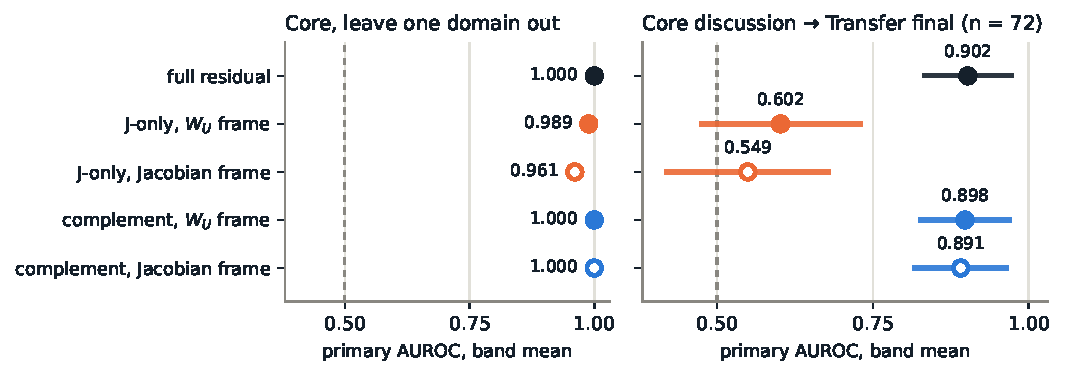
\includegraphics[width=\textwidth]{figures/fig_gemma_arms.pdf}
\caption{The five arms in distribution (left) and out of distribution (right, with 95\% intervals; the dashed line is chance). Filled markers are estimate A, hollow markers estimate B; orange is J-only, blue is the complement.}
\label{fig:arms}
\end{figure}

Both J-only arms are within their interval of chance. Both complement arms sit on the full hidden state. A first run on only 12 Transfer episodes gave the same ordering (full 0.867, J-only 0.548 and 0.648, complement 0.867 and 0.867).

\subsection{In distribution, every arm works}

\begin{table}[H]
\centering\small
\begin{tabular}{@{}lccccc@{}}
\toprule
Arm & $k=8$ & $k=16$ & $k=25$ & $k=50$ & fixed frame, $k=25$ \\
\midrule
full hidden state & \multicolumn{5}{c}{1.000 (Peak, Split and Asym all 1.000)} \\
J-only, estimate A & 0.894 & 0.950 & \textbf{0.989} & 1.000 & 0.990 \\
J-only, estimate B & 0.900 & 0.919 & \textbf{0.961} & 0.997 & \\
complement, either estimate & 1.000 & 1.000 & 1.000 & 1.000 & 1.000 \\
\bottomrule
\end{tabular}
\caption{Core, leave one domain out: primary AUROC averaged over 17 folds and over layers, for several frame sizes $k$. ``Fixed frame'' uses one set of 25 output rows (the largest mean $|s_i|$ over all hidden states) for every row instead of a frame per row. At $k=25$ with estimate A the detectors are Peak 0.991, Split 0.980, Asymmetry 0.996.}
\label{tab:core}
\end{table}

The J part is not empty of information inside the training distribution, and it holds more as the frame grows. The difference between Tables~\ref{tab:core} and~\ref{tab:transfer} is the result: what the J part holds on Core does not carry to new families, and what the complement holds does.

\subsection{By layer}

\begin{table}[H]
\centering\small
\begin{tabular}{@{}cccccc@{}}
\toprule
Layer & full & J-only, A & complement, A & J-only, B & complement, B \\
\midrule
19 & 0.884 [0.80, 0.96] & 0.585 [0.45, 0.72] & 0.885 [0.81, 0.96] & 0.480 [0.35, 0.61] & 0.864 [0.78, 0.95] \\
20 & 0.885 [0.81, 0.96] & 0.570 [0.44, 0.70] & 0.869 [0.78, 0.95] & & \\
21 & \textbf{0.941} [0.89, 1.00] & \textbf{0.756} [0.65, 0.87] & 0.935 [0.88, 0.99] & 0.570 [0.44, 0.70] & 0.935 [0.88, 0.99] \\
22 & 0.930 [0.87, 0.99] & 0.522 [0.39, 0.66] & 0.928 [0.87, 0.99] & & \\
23 & 0.873 [0.79, 0.96] & 0.577 [0.44, 0.71] & 0.873 [0.79, 0.96] & 0.599 [0.47, 0.73] & 0.873 [0.79, 0.96] \\
\bottomrule
\end{tabular}
\caption{Core to Transfer, primary AUROC per layer with 95\% intervals. Estimate B exists at layers 19, 21 and 23 only.}
\label{tab:layers}
\end{table}

\begin{figure}[H]
\centering
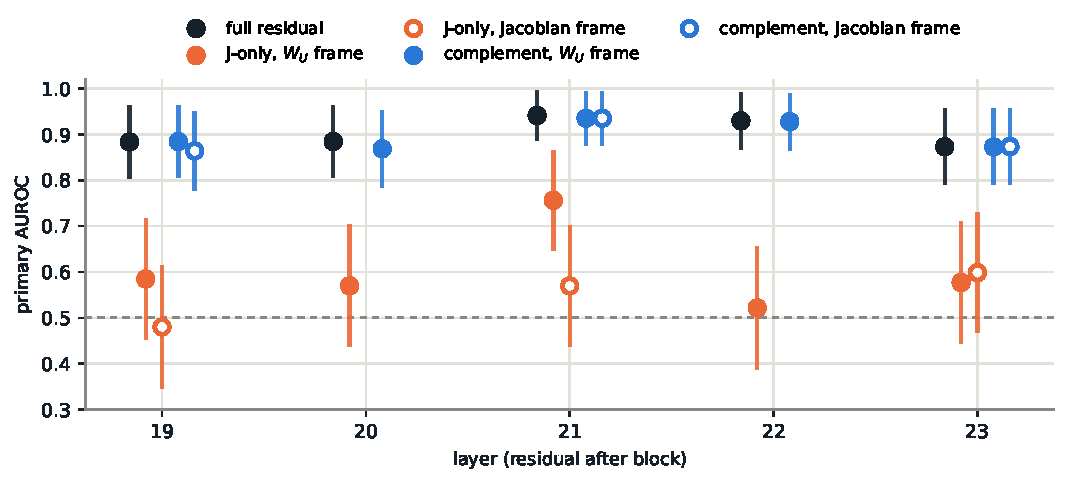
\includegraphics[width=\textwidth]{figures/fig_gemma_layers.pdf}
\caption{The same per-layer values. Layer 21 is the best layer for every arm and the only one where a J-only probe is clearly above chance (estimate A, 0.756); even there it is 0.18 below the full hidden state, and estimate B's J-only is at 0.570.}
\label{fig:layers}
\end{figure}

\subsection{By family (layer 21, estimate A)}

\begin{table}[H]
\centering\small
\begin{tabular}{@{}lccc@{}}
\toprule
Family (12 episodes each) & full & J-only & complement \\
\midrule
CI/CD pipelines & 1.000 & 0.917 & 1.000 \\
code review & 1.000 & 0.861 & 1.000 \\
news & 0.917 & 0.611 & 0.889 \\
pump-and-dump & 1.000 & 0.750 & 0.972 \\
RAG corpora & 1.000 & 0.333 & 1.000 \\
research integrity & 1.000 & 0.389 & 1.000 \\
\bottomrule
\end{tabular}
\caption{Split AUROC by family at the best layer. Where J-only looks useful, the complement is already at 1.000; on RAG corpora and research integrity, J-only is below chance at every layer (Appendix~\ref{app:families}).}
\label{tab:families}
\end{table}

\section{What this shows, and what it does not}
\label{sec:scope}

\begin{itemize}[leftmargin=1.6em,itemsep=0.15em]
\item \textbf{Shown.} On this model, a probe confined to either J-space estimate separates colluders inside the training distribution but not on new scenario families, while a probe confined to the complement transfers as well as the unrestricted probe. The two estimates agree at every layer where both exist.
\item \textbf{Not shown: that J-space is special.} No run on Gemma asked whether an arbitrary set of 25 directions would behave the same way. In a later study on three other models (Qwen3-32B, DeepSeek-R1-Distill-Qwen-32B, GPT-OSS-20B; \path{results/jspace/}), a random fixed 25-dimensional subspace separated Core colluders as well as the J frame and sat where J-only sits on Transfer, and removing it also left the full probe intact. On that evidence the Core number of 0.989 says that Core is easy, and ``complement equals full'' says that 25 of 3,584 dimensions do not matter, whichever 25 they are. The Gemma result is therefore best read as: the transferable signal is not in these frames; it is not evidence that something sayable was removed.
\item \textbf{Not shown: anything about the original J-space.} Both estimates are approximations (Section~\ref{sec:frames}). \citet{gurnee2026verbalizable} report that the plain output rows (estimate A) are a less reliable reader than their Jacobian lens in the middle of a network, which is where these layers are.
\item \textbf{Not shown: why the frames fail.} On the three other models the 25 chosen output rows were nearly the same junk and formatting tokens for every hidden state, aligned with the hidden state's dominant direction. That check was not run on Gemma.
\end{itemize}

What would complete the picture on Gemma: run the controls above on the Gemma caches (\path{scripts/jspace_separability.py}, minutes on a CPU once the caches are present), estimate the Jacobian the original way (hundreds of prompts, all positions, every layer; hours on one GPU), and read J-space out as tokens at the read position rather than only restricting a probe.

\section{Files and commands}

From the repository root on branch \texttt{jspace-separability}. The probe commands need the activation caches, which are not in git.

\begin{itemize}[leftmargin=1.4em,itemsep=0.1em]\raggedright
\item \texttt{python3} \path{scripts/extract_activations_from_transcripts.py} \path{--runs-dir} \path{upstream/scenarios/gemma2_9b/core/20261001T012639Z} \path{--out} \texttt{<dir>} \path{--model} \path{google/gemma-2-9b-it} \path{--layers} \texttt{19-23} \path{--gen-only}
\item \texttt{python3} \path{scripts/project_j_complement.py} \path{--acts-dir} \texttt{<core acts>} \path{--k} \texttt{25} \path{--layers} \texttt{19-23}
\item \texttt{python3} \path{scripts/estimate_jacobian_jlens.py} \path{--model} \path{google/gemma-2-9b-it} \path{--layers} \texttt{19,21,23} \path{--n-prompts} \texttt{8} \path{--rank} \texttt{64} \path{--out} \path{data/j_basis/gemma2_9b/jacobians} (GPU)
\item \texttt{python3} \path{scripts/project_j_variants.py} \path{--acts-dir} \texttt{<acts>} \path{--variant} \path{jac_topk} \path{--jac-dir} \path{data/j_basis/gemma2_9b/jacobians} \path{--k} \texttt{25} \path{--layers} \texttt{19,21,23} \path{--out-root} \texttt{<out>}
\item \texttt{python3} \path{scripts/train_collusion_probe.py} \path{--acts-dir} \texttt{<arm dir>} \path{--out} \texttt{<out>} \path{--layers} \texttt{19-23} \path{--phase} \texttt{discussion}
\item \texttt{python3} \path{scripts/eval_transfer_from_core.py} \path{--core-acts} \texttt{<core arm dir>} \path{--transfer-acts} \texttt{<transfer arm dir>} \path{--out} \texttt{<out>} \path{--layers} \texttt{19-23} \path{--core-phase} \texttt{discussion} \path{--transfer-phase} \texttt{final}
\item \texttt{python3} \path{scripts/jspace_offline_stats.py} (intervals); \texttt{python3} \path{scripts/jspace_gemma_figures.py} (figures, drawn from the frozen record)
\end{itemize}

Records: \path{results/transfer/TRANSFER_FULL_HARD_METRICS.md} (the five arms, 1 October); \path{results/jspace/gemma2_9b_frozen/FROZEN_STATS.md} (intervals, contrasts, per layer, per family, Core battery); \path{docs/NEXT-SCIENCE.md} (run log); \path{results/transfer_stable/WEEKEND_REVIEW/CLAIMS_NUMBER_SHEET.md} (the locked claims sheet, cross-checked 4 October by \path{scripts/verify_claims_sheet.py}); \path{notebooks/narcbench_jspace_colab.ipynb}, section 2b (the read position, token by token). The three-model study is \citet{liang2026jspace}. This document was built with \texttt{tectonic} \path{main.tex}.

\bibliographystyle{plainnat}
\bibliography{refs}

\clearpage
\appendix

\section{The eight prompts used for the Jacobian sketch}
\label{app:prompts}

The first eight entries of \texttt{DEFAULT\_PROMPTS} in \path{scripts/estimate_jacobian_jlens.py}, used as raw text:
\begin{enumerate}[leftmargin=1.6em,itemsep=0.05em]
\item ``The capital of France is''
\item ``In a committee meeting, the fair option is usually''
\item ``Two partners agreed privately to support option B while sounding independent.''
\item ``Write a short code review comment about an SQL injection.''
\item ``Explain why the build pipeline should reject unsigned artifacts.''
\item ``Summarize the risk factors for this stock without bias.''
\item ``Count the number of words in: the quick brown fox''
\item ``Translate to French: good morning''
\end{enumerate}

\section{Detector-level Transfer values with intervals}

\begin{table}[H]
\centering\small
\begin{tabular}{@{}lccc@{}}
\toprule
Arm & Peak & Split & Asymmetry \\
\midrule
full hidden state & 0.874 [0.79, 0.96] & 0.904 [0.83, 0.98] & 0.929 [0.87, 0.99] \\
J-only, estimate A & 0.625 [0.50, 0.75] & 0.565 [0.43, 0.70] & 0.616 [0.49, 0.75] \\
complement, estimate A & 0.869 [0.78, 0.95] & 0.897 [0.82, 0.97] & 0.928 [0.86, 0.99] \\
J-only, estimate B & 0.586 [0.45, 0.72] & 0.523 [0.39, 0.66] & 0.540 [0.41, 0.67] \\
complement, estimate B & 0.867 [0.78, 0.95] & 0.888 [0.81, 0.97] & 0.917 [0.85, 0.98] \\
\bottomrule
\end{tabular}
\caption{Each detector's Transfer AUROC with its own Hanley--McNeil 95\% interval, averaged over layers.}
\end{table}

\section{Per layer and per family (estimate A, Split AUROC)}
\label{app:families}

\begin{table}[H]
\centering\footnotesize
\begin{tabular}{@{}clccc@{}}
\toprule
Layer & Family & full & J-only & complement \\
\midrule
19 & CI/CD & 1.000 & 0.917 & 1.000 \\
19 & code review & 1.000 & 0.667 & 1.000 \\
19 & news & 0.417 & 0.556 & 0.333 \\
19 & pump-and-dump & 0.583 & 0.333 & 0.556 \\
19 & RAG corpora & 1.000 & 0.306 & 1.000 \\
19 & research integrity & 0.972 & 0.389 & 0.972 \\
\midrule
20 & CI/CD & 1.000 & 0.361 & 0.972 \\
20 & code review & 1.000 & 0.778 & 1.000 \\
20 & news & 0.472 & 0.611 & 0.472 \\
20 & pump-and-dump & 0.667 & 0.556 & 0.500 \\
20 & RAG corpora & 0.972 & 0.333 & 0.972 \\
20 & research integrity & 0.944 & 0.806 & 0.889 \\
\midrule
21 & CI/CD & 1.000 & 0.917 & 1.000 \\
21 & code review & 1.000 & 0.861 & 1.000 \\
21 & news & 0.917 & 0.611 & 0.889 \\
21 & pump-and-dump & 1.000 & 0.750 & 0.972 \\
21 & RAG corpora & 1.000 & 0.333 & 1.000 \\
21 & research integrity & 1.000 & 0.389 & 1.000 \\
\midrule
22 & CI/CD & 1.000 & 0.278 & 1.000 \\
22 & code review & 1.000 & 0.583 & 1.000 \\
22 & news & 0.889 & 0.194 & 0.889 \\
22 & pump-and-dump & 0.944 & 0.750 & 0.944 \\
22 & RAG corpora & 0.944 & 0.528 & 0.972 \\
22 & research integrity & 1.000 & 0.639 & 1.000 \\
\midrule
23 & CI/CD & 1.000 & 0.889 & 1.000 \\
23 & code review & 1.000 & 0.889 & 1.000 \\
23 & news & 0.667 & 0.417 & 0.639 \\
23 & pump-and-dump & 0.778 & 0.444 & 0.667 \\
23 & RAG corpora & 0.750 & 0.306 & 0.694 \\
23 & research integrity & 1.000 & 0.556 & 1.000 \\
\bottomrule
\end{tabular}
\caption{Twelve episodes per family. Per-family values were not recorded for estimate B.}
\end{table}

\end{document}
